\documentclass{report}
\usepackage[utf8]{inputenc}
\usepackage[italian]{babel}
\usepackage[a4paper, left=2.5cm, right=2.5cm]{geometry}
\usepackage[hidelinks]{hyperref}
\usepackage{graphicx}
\graphicspath{ {./img/} }


\begin{document}

	\centerline{
\includegraphics{logo}}
	\bigbreak

	\begin{center}
		Corso di
        \vskip 0.2cm
		\large{\textbf{Programmazione Logica e Funzionale}}
		\vskip 2cm
		Anno accademico
        \vskip 0.2cm
 		\textbf{2021-2022}
		\vskip 2cm
		Progetto realizzato da
        \vskip 0.2cm
		\textbf{Barzotti Cristian}
        \vskip 0.1cm 290725
        \vskip 0.2cm
        \textbf{Kania Nicholas} 
        \vskip 0.1cm 
        291188
		\vfill
		Corso tenuto dal professore
        \vskip 0.2cm
		\large{\textbf{Bernardo Marco}}
	\end{center}
	
	\part*{Implementazione di DCT e DFT in Haskell e Prolog}
	\tableofcontents % Indice

	
	\chapter{Specifica del problema}
	Si propone di implementare le funzioni denominate DCT
	(\textit{Discrete Cosine Transform}) e DFT (\textit{Discrete Fourier Transform}), 
	e le relative funzioni inverse IDCT e IDFT. \\
	\section*{Nota}
	Ci teniamo a precisare che la funzione DCT è suddivisa in diversi tipi; in questo progetto siamo andati ad implementare quelle che formalmente sono chiamate DCT tipo II e DCT tipo III\footnote{\url{https://en.wikipedia.org/wiki/Discrete_cosine_transform}}.\\ 
	In questo progetto, e relativa documentazione, ci riferiremo alle funzioni rispettivamente come DCT (per la funzione DCT tipo II) e IDCT (per la funzione DCT tipo III).
	
	\chapter{Analisi del problema}
	% Il programma prevede l'inserimento di due array di numeri; il primo array verrà richiesto all'avvio del programma per il calcolo di DCT e IDCT, mentre il secondo array verrà richiesto una volta effettuati i dovuti calcoli sul primo array e sarà utilizzato per calcolare DFT e IDFT.

	
	\section{Dati di ingresso del problema}
	
	\begin{itemize}
		\item una lista di numeri reali per il calcolo di DCT e IDCT;
		\item una lista di numeri complessi per il calcolo di DFT e IDFT.
	\end{itemize}
	\section{Dati di uscita del problema}
	\begin{itemize}
		\item una lista di numeri reali calcolati con DCT;
		\item una lista di numeri reali calcolati con IDCT;
		\item una lista di numeri complessi calcolato con DFT;
		\item una lista di numeri complessi calcolato con IDFT.
	\end{itemize}
	\section{Relazioni intercorrenti tra i dati del problema}
  Tutte le formule che andremo ad utilizzare all'interno del programma seguono la seguente logica:
  data una sequenza di numeri iniziale di lunghezza $N$, verrà creata una nuova sequenza di numeri anch'essa di lunghezza $N$.
  Tutte le formule sono state prese dagli appunti del corso di Elaborazione Segnali ed Immagini.\footnote{\url{https://blended.uniurb.it/moodle/mod/folder/view.php?id=102652}}
  \subsection{DCT}
  Utilizzando la \textit{Discrete Cosine Transform} su una sequenza di numeri reali, il $k$-esimo elemento sarà calcolato con la seguente formula:
  \[C(k) = 2 \sum_{n = 0}^{N -1} x(n) cos\left[\frac{\pi(2n + 1)k}{2N}\right]\].
  
  \subsection{IDCT}
  Utilizzando la \textit{Inverse Discrete Cosine Transform} su una sequenza di numeri reali, l' $n$-esimo elemento sarà calcolato con la seguente formula:
  \[x(n) = \frac{1}{2N}\left\{C(0) + \sum_{k = 1}^{N -1} 2C(k) cos\left[\frac{\pi(2n + 1)k}{2N}\right]\right\}\]
  \noindent La sequenza di numeri iniziali con cui calcolare la \textit{IDCT} verrà presa dall'output della \textit{DCT} e, a meno di errori di approssimazione, sarà uguale alla sequenza di numeri utilizzata per il calcolo della \textit{DCT}.

  \subsection{DFT}
  Utilizzando la \textit{Discrete Fourier Transform} su una sequenza di numeri complessi, il $k$-esimo elemento sarà calcolato con la seguente formula:
  \[X_p(k) = \sum_{n = 0}^{N -1} x_p(n)e^{-j\frac{2\pi}{N}nk}\].
  
  \subsection{IDFT}
  Utilizzando la \textit{Inverse Discrete Fourier Transform} su una sequenza di numeri complessi, l' $n$-esimo elemento sarà calcolato con la seguente formula:
  \[x_p(n) = \frac{1}{N}\sum_{k = 0}^{N -1} X_p(k) e^{j\frac{2\pi}{N}nk}\]
  \noindent La sequenza di numeri iniziali con cui calcolare la \textit{IDFT} verrà presa dall'output della \textit{DFT} e, a meno di errori di approssimazione, sarà uguale alla sequenza di numeri utilizzata per il calcolo della \textit{DFT}.
	
	\chapter{Progettazione dell'algoritmo}
	\section{Scelte di progetto}
  Per rendere più intuitiva l'implementazione, abbiamo deciso di utilizzare la forma cartesiana dei numeri complessi al posto della forma esponenziale, sostituendo $e^{-j\frac{2\pi}{N}nk}$ con la forma cartesiana $cos(\theta) + j sin(\theta)$, dove $\theta = -\frac{2\pi}{N}nk$.\\
  \noindent Tutti gli input del programma sono liste di numeri e andranno inseriti in maniera opportuna, in base al linguaggio utilizzato. 
  \subsection{Haskell}
  Per i numeri reali, la lista deve essere inserita nel formato:
  \[[<numero>, ...]\footnote{es: [1, 0.5, -3]}\]
  \vskip 0.1cm
  \noindent Per i numeri complessi, la lista deve essere inserita nel formato:
  \[[<parte\ reale> :+ <parte\ immaginaria>, ...]\footnote{es: [1 :+ 2, 0.5 :+ -3, 0 :+ 0]}\]

  \subsection{Prolog}
  Per i numeri reali, la lista deve essere inserita nel formato:
  \[[<numero>, ...].\footnote{es: [1, 0.5, -3].}\]
  \vskip 0.1cm
  \noindent Per i numeri complessi, la lista deve essere inserita nel formato:
  \[[(<parte\ reale>, <parte\ immaginaria>), ...].\footnote{es: [(1,2), (0.5,-3), (0,0)].}\]

  \newpage
	\section{Passi dell'algoritmo}
	I passi dell'algoritmo da eseguire per ogni trasformata sono i seguenti:

  \begin{itemize}
    \item chiama la funzione di generazione della lista sull'elemento di indice $k$;
		\begin{itemize}
      \item chiama la funzione di generazione della lista sull'elemento $k+1$ fino al caso base;
      \item calcola il $k$-esimo elemento;
      \begin{itemize}
        \item somma ricorsivamente i valori della lista;
      \end{itemize}
      \item lo aggiunge in testa alla lista;
      \item restituisce la lista;
    \end{itemize} 

  \end{itemize}

  \noindent Per semplicità di lettura, rinominiamo i precedenti passi come \textbf{\textit{calcolo della trasformata}}.
  I passi dell'algoritmo del nostro programma diventeranno quindi:

	\begin{itemize}
		\item inserimento di una lista di numeri reali da tastiera per il calcolo della DCT;
    \item \textbf{\textit{calcolo della trasformata}} DCT;
    \item stampa della lista;
    \item \textbf{\textit{calcolo della trasformata}} IDCT, con il precedente output come valori di input;
    \item stampa della lista;
		\item inserimento di una lista di numeri complessi da tastiera per il calcolo della DFT;
    \item \textbf{\textit{calcolo della trasformata}} DFT;
    \item stampa della lista;
    \item \textbf{\textit{calcolo della trasformata}} IDFT, con il precedente output come valori di input;
    \item stampa della lista.


	\end{itemize}
	
	\chapter{Implementazione dell'algoritmo}
	\section{Haskell}

	\small
	{\fontfamily{pcr}\selectfont
	\begin{verbatim}
{- IMPORTAZIONE DELLE LIBRERIE -}
{- Libreria necessaria per utilizzare la funzione 'length' -}
import Data.List
{- Libreria utilizzata per la gestione dei numeri complessi -}
import Data.Complex
{- Libreria necessaria per:
    - utilizzare il tipo 'Either';
    - utilizzare la funzione 'readEither' -}
import Text.Read



{- MAIN -}
{- Il programma accetta in input una lista di numeri reali,
    calcolandone e stampandone i risultati:
      - la trasformata discreta del coseno (DCT);
      - relativa trasformata inversa (IDCT).
    
    Viene poi richiesta in input una lista di numeri complessi,
    calcolandone e stampandone i risultati:
      - la trasformata discreta di Fourier (DFT);
      - relativa trasformata inversa. -}
main :: IO()
main = do
  putStrLn "Progetto della sessione autunnale del corso Programmazione Logica e Funzionale"
  putStrLn "Anno 2021/2022"
  putStrLn "Corso tenuto dal prof. Marco Bernardo"
  putStrLn "Progetto realizzato da: Barzotti Cristian e Kania Nicholas\n\n"


  real_list <- acquire_real_list
  let val_dct = dct real_list
  
  putStrLn "\nDCT:"
  putStrLn $ show val_dct
  putStr "\n"
  putStrLn "IDCT:"
  putStrLn $ show (idct val_dct)

  putStr "\n\n"

  complex_list <- acquire_complex_list
  
  let val_dft = dft complex_list
  
  putStrLn "\nDFT:"
  putStrLn $ show val_dft
  putStr "\n"
  putStrLn "IDFT:"
  print (stringify_complex_list (idft val_dft))



{- DCT -}
{- Funzione per il calcolo della DCT -}
dct :: [Double] -> [Double]
dct [] = []
dct xs = generate_dct xs (length xs) 0

{- Genera la trasformata -}
generate_dct :: [Double] -> Int -> Int -> [Double]
generate_dct [] _ _ = []
generate_dct xs size k
  | k == size = []
  | otherwise = 
    (sum_terms_dct xs size k 0) : 
    (generate_dct xs size (k + 1))

{- Effettua il calcolo del k-esimo elemento della trasformata -}
sum_terms_dct :: [Double] -> Int -> Int -> Int -> Double
sum_terms_dct [] _ _ _ = 0.0
sum_terms_dct (x:xs) size k n =
  2 * x * 
  cos (pi *  fromIntegral ((2 * n + 1) * k) / fromIntegral (2 * size)) + 
  sum_terms_dct xs size k (n + 1)



{- IDCT -}
{- Funzione per il calcolo della IDCT -}
idct :: [Double] -> [Double]
idct [] = []
idct xs = generate_idct xs (length xs) 0

{- Genera la trasformata inversa (serie originale) -}
generate_idct :: [Double] -> Int -> Int -> [Double]
generate_idct [] _ _ = []
generate_idct (x:xs) size n
  | n == size = []
  | otherwise = 
    ((x + sum_terms_idct xs size n 1) / fromIntegral (2 * size)) : 
    (generate_idct (x:xs) size (n + 1))

{- Effettua il calcolo della sommatoria per k-esimo elemento della trasformata inversa -}
sum_terms_idct :: [Double] -> Int -> Int -> Int -> Double
sum_terms_idct [] _ _ _ = 0.0
sum_terms_idct (x:xs) size n k =
  2 * x * 
  cos (pi *  fromIntegral ((2 * n + 1) * k) / fromIntegral (2 * size)) + 
  sum_terms_idct xs size n (k + 1)



{- DFT -}
{- Funzione per il calcolo della DFT -}
dft :: [Complex Double] -> [Complex Double]
dft [] = []
dft xs = generate_dft xs (length xs) 0

{- Genera la trasformata -}
generate_dft :: [Complex Double] -> Int -> Int -> [Complex Double]
generate_dft [] _ _ = []
generate_dft xs size k
  | k == size = []
  | otherwise = 
    (sum_terms_dft xs size k 0) : 
    (generate_dft xs size (k + 1))

{- Effettua il calcolo del k-esimo elemento della trasformata -}
sum_terms_dft :: [Complex Double] -> Int -> Int -> Int -> Complex Double
sum_terms_dft [] _ _ _ = 0.0
sum_terms_dft (x:xs) size k n =
  let
    theta = - ((2.0 * pi) / (fromIntegral size)) * (fromIntegral n) * (fromIntegral k)
  in
    (x * (cos theta :+ sin theta)) + sum_terms_dft xs size k (n + 1)



{- IDFT -}
{- Funzione per il calcolo della IDFT -}
idft :: [Complex Double] -> [Complex Double]
idft [] = []
idft xs = generate_idft xs (length xs) 0

{- Genera la trasformata inversa (serie originale) -}
generate_idft :: [Complex Double] -> Int -> Int -> [Complex Double]
generate_idft [] _ _ = []
generate_idft xs size n
  | n == size = []
  | otherwise = 
    (sum_terms_idft xs size n 0 / (fromIntegral size)) : 
    (generate_idft xs size (n + 1))

{- Calcolo della sommatoria per il k-esimo elemento -}
sum_terms_idft :: [Complex Double] -> Int -> Int -> Int -> Complex Double
sum_terms_idft [] _ _ _ = 0.0
sum_terms_idft (x:xs) size n k =
  let
    theta = ((2.0 * pi) / (fromIntegral size)) * (fromIntegral n) * (fromIntegral k)
  in
    (x * (cos theta :+ sin theta)) + sum_terms_idft xs size n (k + 1)



{- FUNZIONI AUSILIARIE -}
{- Converte una lista di numeri complessi in lista di stringhe -}
stringify_complex_list :: [Complex Double] -> [String]
stringify_complex_list [] = []
stringify_complex_list (x:xs) = (show x) : (stringify_complex_list xs)


{- Acquisisce una lista di numeri reali da tastiera.
    La funzione non termina fino a quando non verrà inserita una lista valida. -}
acquire_real_list :: IO [Double]
acquire_real_list = do
  putStrLn "Inserisci una lista di numeri reali nel formato:\n"
  putStrLn "\t[<numero>, ...]\n"
  putStrLn "Per esempio: [1, 0.5, -3]"
  line <- getLine
  
  case readEither line :: Either String [Double] of
    Left err -> do
      putStrLn "\nErrore."
      acquire_real_list
    Right value -> return (value)


{- Acquisisce una lista di numeri complessi da tastiera.
    La funzione non termina fino a quando non verrà inserita una lista valida. -}
acquire_complex_list :: IO [Complex Double]
acquire_complex_list = do
  putStrLn "Inserisci una lista di numeri complessi nel formato:\n"
  putStrLn "\t[<parte reale> :+ <parte immaginaria>, ...]\n"
  putStrLn "Per esempio: [1 :+ 2, 0.5 :+ -3, 0 :+ 0]"
  line <- getLine
  
  case readEither line :: Either String [Complex Double] of
    Left err -> do
      putStrLn "\nErrore."
      acquire_complex_list
    Right value -> return (value)
  \end{verbatim}
	}
	\normalsize

	

  \section{Prolog}
	\small
	{\fontfamily{pcr}\selectfont
	\begin{verbatim}
/* MAIN */
/* Il programma accetta in input una lista di numeri reali,
   calcolandone e stampandone i risultati:
     - la trasformata discreta del coseno (DCT);
     - relativa trasformata inversa (IDCT).
   
   Viene poi richiesta in input una lista di numeri complessi,
   calcolandone e stampandone i risultati:
     - la trasformata discreta di Fourier (DFT);
     - relativa trasformata inversa. */
main :-
  nl,
  write('Progetto della sessione autunnale del corso Programmazione Logica e Funzionale'), nl,
  write('Anno 2021/2022'), nl,
  write('Corso tenuto dal prof. Marco Bernardo'), nl,
  write('Progetto realizzato da: Barzotti Cristian e Kania Nicholas'), nl, nl, nl,

  acquire_real_list(RealList), nl,
  dct(RealList, C),
  write('DCT:'), nl,
  write(C), nl, nl,
  idct(C, DctOriginal),
  write('IDCT:'), nl,
  write(DctOriginal), nl, nl,nl,
  
  acquire_complex_list(ComplexList), nl,
  dft(ComplexList, X),
  write('DFT:'), nl,
  write(X), nl, nl,
  idft(X, DftOriginal),
  write('IDFT:'), nl,
  write(DftOriginal), nl.



/* DCT */
/* Funzione per il calcolo della DCT */
dct([], []).
dct([X | Y], C) :-  
  size([X | Y], S),
  generate_dct([X | Y], S, 0, C).
                    
/* Genera la trasformata */
generate_dct([], _, _, []).
generate_dct(L, S, K, C) :- 
  ((K == S) -> 
    C = [];
    K1 is K + 1,
    generate_dct(L, S, K1, C1),
    sum_terms_dct(L, S, K, 0, E),
    append([E], C1, C)).

/* Effettua il calcolo del k-esimo elemento della trasformata */
sum_terms_dct([], _, _, _, 0.0).
sum_terms_dct([H | T], S, K, N, C) :- 
  N1 is N + 1,
  sum_terms_dct(T, S, K, N1, C1),
  C is C1 + (H * 2 * cos(pi * (2 * N + 1) * K / (2 * S))).



/* IDCT */
/* Funzione per il calcolo della IDCT */
idct([], []).
idct([X | Y], C) :- 
  size([X | Y], S),
  generate_idct([X | Y], S, 0, C).

/* Genera la trasformata inversa (serie originale) */                    
generate_idct([], _, _, []).
generate_idct([H | T], S, N, C) :- 
  ((N == S) -> 
    C = [];
    N1 is N + 1,
    generate_idct([H | T], S, N1, C1),
    sum_terms_idct(T, S, N, 1, E),
    X is (H + E) / (2 * S),
    append([X], C1, C)).

/* Effettua il calcolo della sommatoria per k-esimo elemento della trasformata inversa */
sum_terms_idct([], _, _, _, 0.0).
sum_terms_idct([H | T], S, N, K, C) :- 
  K1 is K + 1,
  sum_terms_idct(T, S, N, K1, C1),
  C is C1 + (H * 2 * cos(pi * (2 * N + 1) * K / (2 * S))).



/* DFT */
/* Funzione per il calcolo della DFT */
dft([], []).
dft([X | Y], C) :- 
  size([X | Y], S),
  generate_dft([X | Y], S, 0, C).

/* Genera la trasformata */                 
generate_dft([], _, _, []).
generate_dft(L, S, K, C) :- 
  ((K == S) -> 
    C = [];
    K1 is K + 1,
    generate_dft(L, S, K1, C1),
    sum_terms_dft(L, S, K, 0, E),
    append([E], C1, C)).

/* Effettua il calcolo del k-esimo elemento della trasformata */
sum_terms_dft([], _, _, _, (0,0)).
sum_terms_dft([H | T], S, K, N, C) :- 
  N1 is N + 1,
  THETA is (-((2 * pi) / S) * N * K),
  sum_terms_dft(T, S, K, N1, C1),
  complex_prod(H, (cos(THETA),sin(THETA)), P),
  complex_sum(P, C1, C).



/* IDFT */
/* Funzione per il calcolo della IDFT */
idft([], []).
idft([X | Y], C) :- 
  size([X | Y], S),
  generate_idft([X | Y], S, 0, C).            

/* Genera la trasformata inversa (serie originale) */
generate_idft([], _, _, []).
generate_idft(L, S, N, C) :-
  ((N == S) -> C = [];
  N1 is N + 1,
  generate_idft(L, S, N1, C1),
  sum_terms_idft(L, S, N, 0, E),
  complex_div_real(E, S, P),
  append([P], C1, C)).

/* Calcolo della sommatoria per il k-esimo elemento */
sum_terms_idft([], _, _, _, (0,0)).
sum_terms_idft([H | T], S, N, K, C) :- 
  K1 is K + 1,
  THETA is (((2 * pi) / S) * N * K),
  sum_terms_idft(T, S, N, K1, C1),
  complex_prod(H, (cos(THETA),sin(THETA)), P),
  complex_sum(P, C1, C).



/* FUNZIONI AUSILIARIE */
/* Funzione per calcolare il numero di elementi in una lista */
size([], 0).
size([_ | Y], S) :-
  size(Y, S1),
  S is S1 + 1.

/* Funzione che definisce il prodotto fra numeri complessi */
complex_prod((ZR, ZI), (WR, WI), (R,I)) :-  
  R is (ZR * WR - ZI * WI),
  I is (ZR * WI + ZI * WR).

/* Funzione che definisce la somma fra numeri complessi */
complex_sum((ZR, ZI), (WR, WI), (R,I)) :- 
  R is ZR + WR, 
  I is ZI + WI.

/* Funzione che definisce la divisione fra un numero complesso ed un numero reale */
complex_div_real((ZR, ZI), N, (R, I)) :- 
  R is ZR / N, 
  I is ZI / N.

/* Acquisisce una lista di numeri reali da tastiera.
   La funzione non termina fino a quando non verrà inserita una lista valida. */
acquire_real_list(List) :-
  repeat,
  write('Inserisci una lista di numeri reali nel formato:'), nl, nl,
  write('\t[<numero>, ...].'), nl, nl,
  write('Per esempio: [1, 0.5, -3].'), nl,
  catch(read(List), Error, true),
  ((check_real_list(List), var(Error)) -> 
    !;
    nl, write('Errore.'), nl, fail).

/* Acquisisce una lista di numeri complessi da tastiera.
   La funzione non termina fino a quando non verrà inserita una lista valida. */
acquire_complex_list(List) :-
  repeat,
  write('Inserire una lista di numeri complessi nel formato:'), nl, nl,
  write('\t[(<parte reale>, <parte immaginaria>), ...].'), nl, nl,
  write('Per esempio: [(1,2), (0.5,-3), (0,0)].'), nl,
  catch(read(List), Error, true),
  ((check_complex_list(List), var(Error)) -> 
    !; 
    nl, write('Errore.'), nl, fail).

/* Controlla che una lista sia composta solo da numeri reali */
check_real_list([]).
check_real_list([A | L]) :- 
  ((number(A)) -> 
    check_real_list(L); 
    fail).

/* Controlla che una lista sia composta solo tuple rappresentanti numeri complessi */
check_complex_list([]).
check_complex_list([(A, B) | L]) :- 
  ((number(A), number(B)) -> 
    check_complex_list(L); 
    fail).
  \end{verbatim}
	}
	\normalsize

	\chapter{Testing}
    \section{Haskell}
    \begin{center}
      \begin{figure}[h!]
        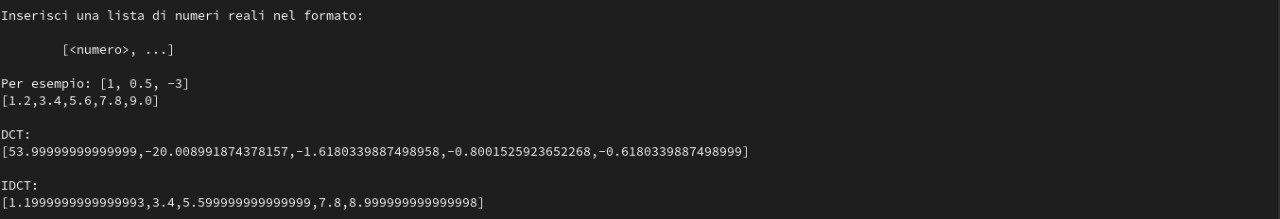
\includegraphics[width=\textwidth]{test_hs_1.jpg}
        \caption{Input corretto durante l'inserimento per DCT}
      \end{figure}
    \end{center}

    \begin{center}
      \begin{figure}[h!]
        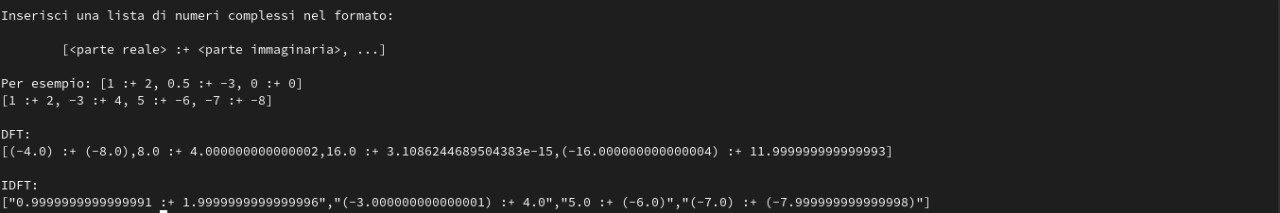
\includegraphics[width=\textwidth]{test_hs_2.jpg}
        \caption{Input corretto durante l'inserimento per DFT}
      \end{figure}
    \end{center}

    \begin{center}
      \begin{figure}
        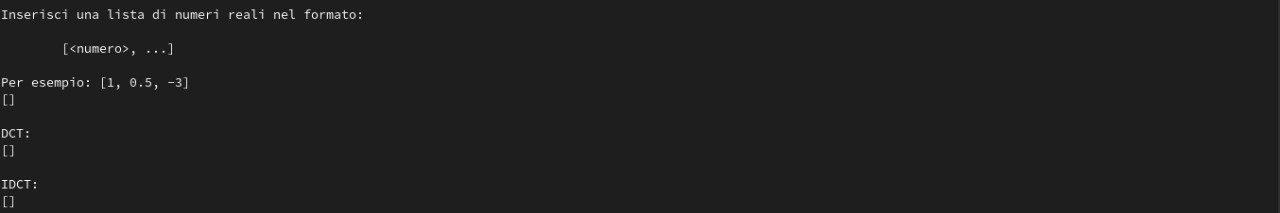
\includegraphics[width=\textwidth]{test_hs_3.jpg}
        \caption{Input vuoto durante l'inserimento per DCT}
      \end{figure}
    \end{center}

    \begin{center}
      \begin{figure}
        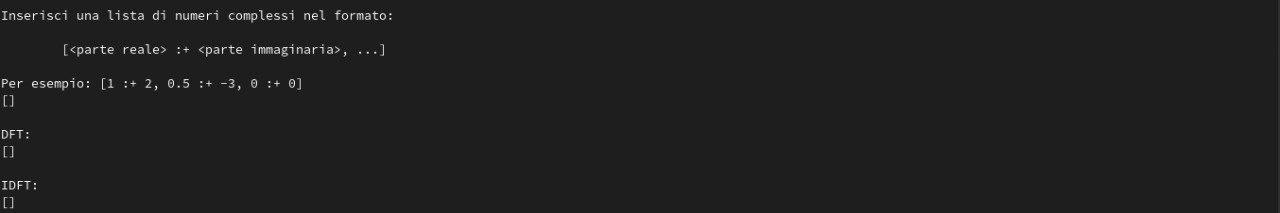
\includegraphics[width=\textwidth]{test_hs_4.jpg}
        \caption{Input vuoto durante l'inserimento per DFT}
      \end{figure}
    \end{center}

    \begin{center}
      \begin{figure}
        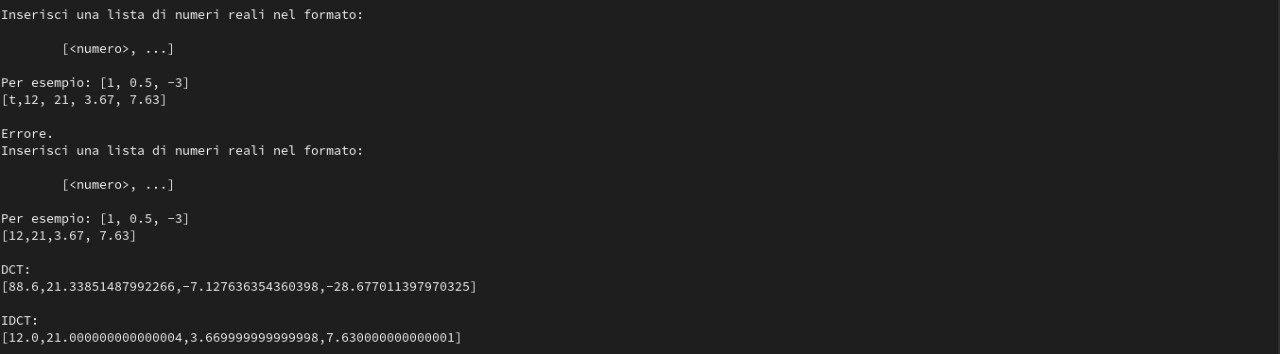
\includegraphics[width=\textwidth]{test_hs_5.jpg}
        \caption{Tipo in input errato durante l'inserimento per DCT}
      \end{figure}
    \end{center}

    \begin{center}
      \begin{figure}
        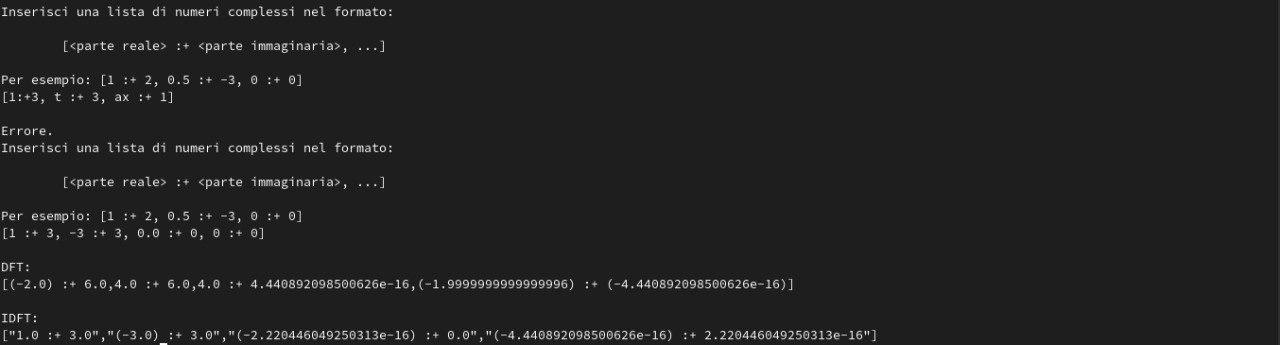
\includegraphics[width=\textwidth]{test_hs_6.jpg}
        \caption{Tipo in input errato durante l'inserimento per DFT}
      \end{figure}
    \end{center}

     \begin{center}
       \begin{figure}
         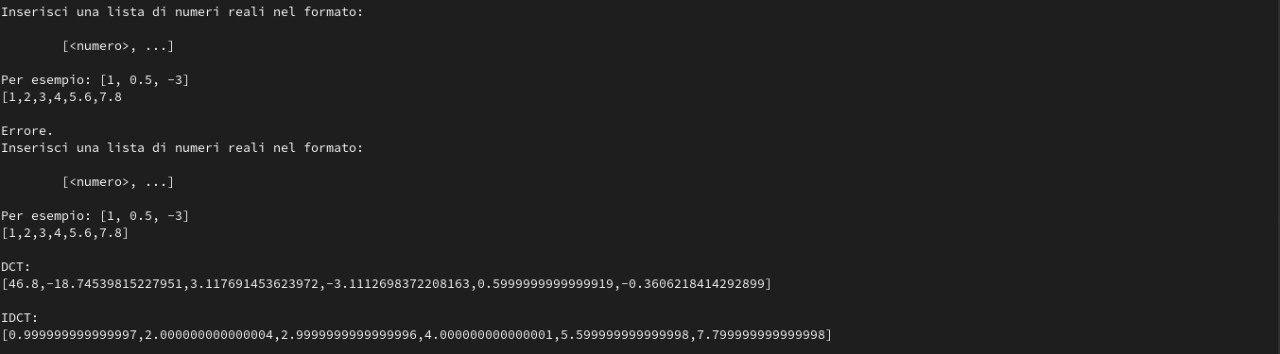
\includegraphics[width=\textwidth]{test_hs_7.jpg}
         \caption{Formattazione errata durante l'inserimento per DCT}
       \end{figure}
     \end{center}

     \begin{center}
       \begin{figure}
         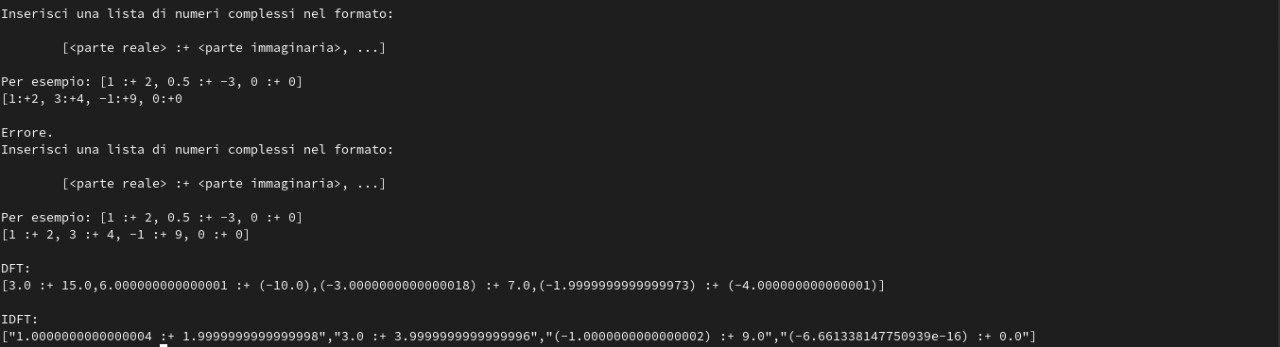
\includegraphics[width=\textwidth]{test_hs_8.jpg}
         \caption{Formattazione errata durante l'inserimento per DFT}
       \end{figure}
     \end{center}

     \begin{center}
       \begin{figure}
         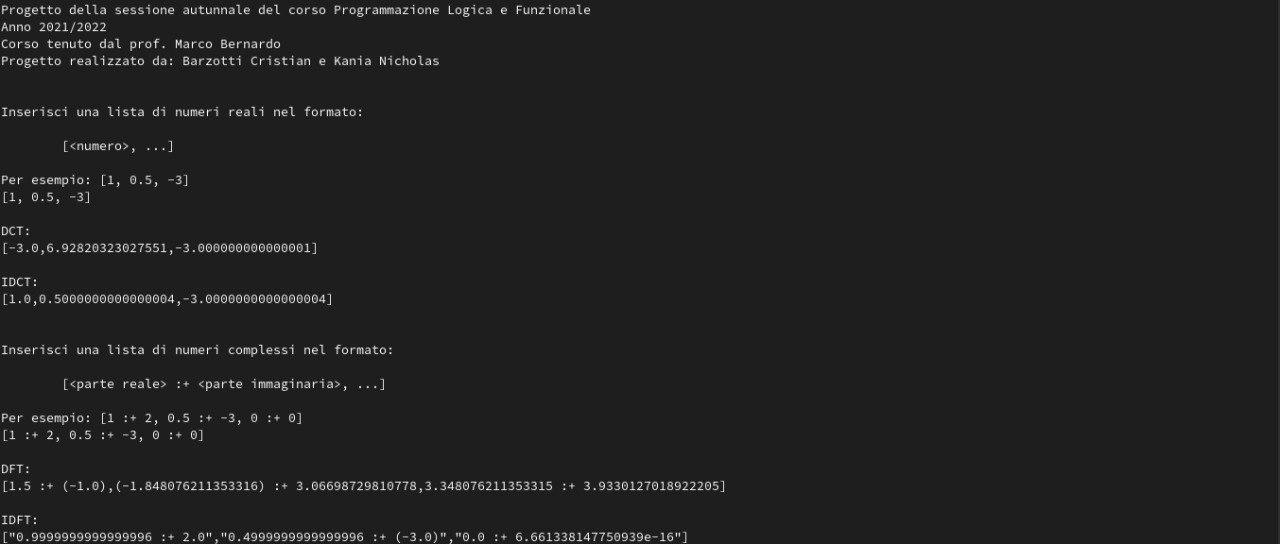
\includegraphics[width=\textwidth]{test_hs_9.jpg}
         \caption{Funzionamento dell'intero programma con input corretti}
       \end{figure}
     \end{center}

     \begin{center}
       \begin{figure}
         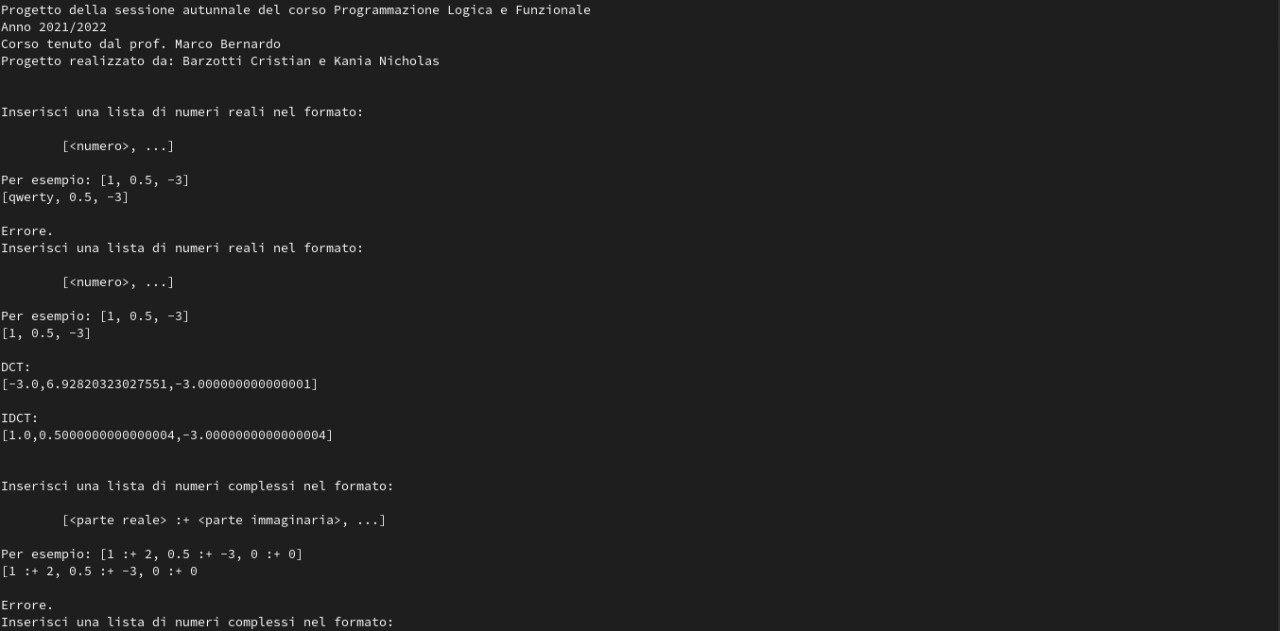
\includegraphics[width=\textwidth]{test_hs_10a.jpg}
         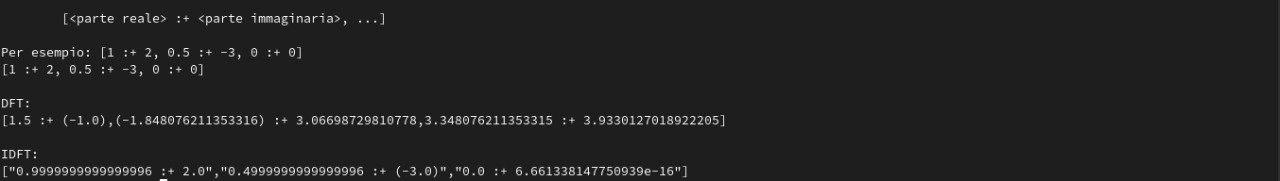
\includegraphics[width=\textwidth]{test_hs_10b.jpg}
         \caption{Funzionamento dell'intero programma con alcuni input errati}
       \end{figure}
     \end{center}


     \newpage
     \section{Prolog}
     \begin{center}
      \begin{figure}[h!]
        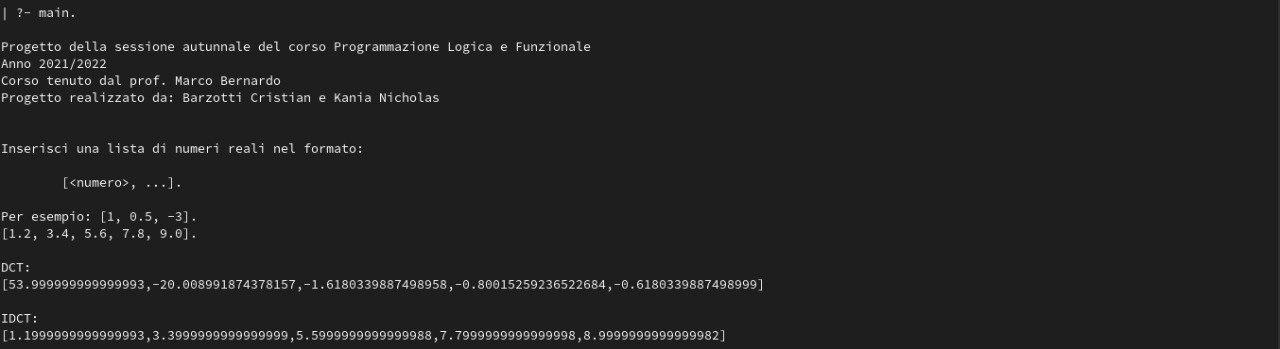
\includegraphics[width=\textwidth]{test_pl_1.jpg}
        \caption{Input corretto durante l'inserimento per DCT}
      \end{figure}
    \end{center}

    \begin{center}
      \begin{figure}[h!]
        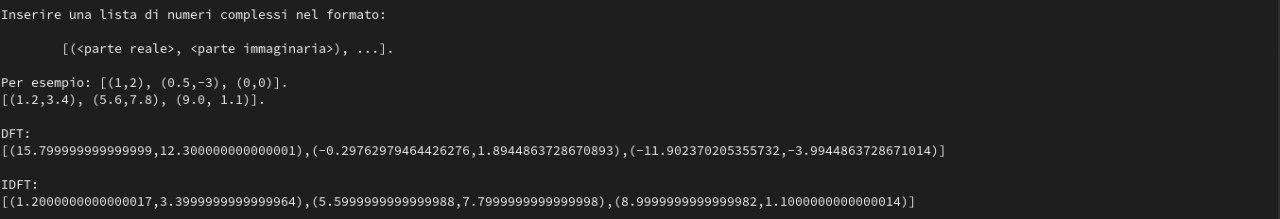
\includegraphics[width=\textwidth]{test_pl_2.jpg}
        \caption{Input corretto durante l'inserimento per DFT}
      \end{figure}
    \end{center}

    \begin{center}
      \begin{figure}
        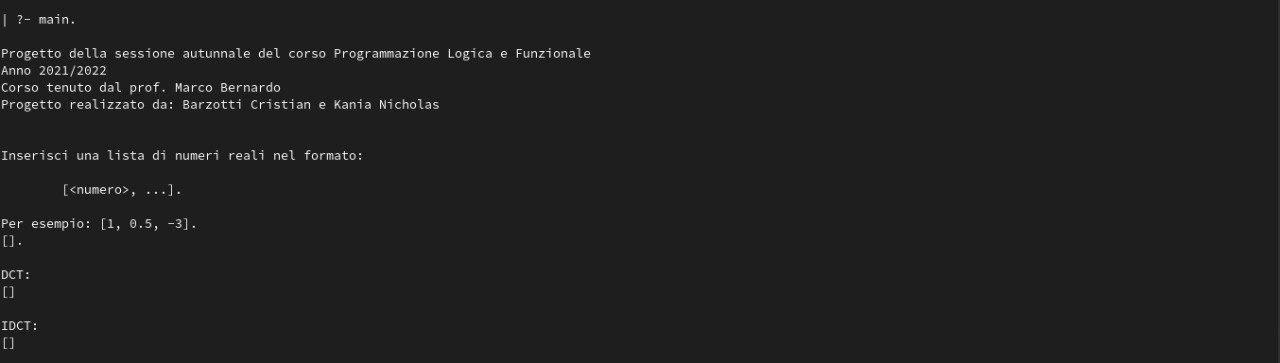
\includegraphics[width=\textwidth]{test_pl_3.jpg}
        \caption{Input vuoto durante l'inserimento per DCT}
      \end{figure}
    \end{center}

    \begin{center}
      \begin{figure}
        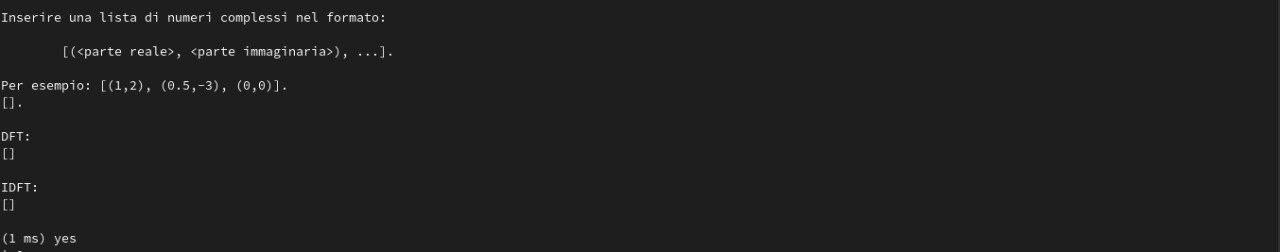
\includegraphics[width=\textwidth]{test_pl_4.jpg}
        \caption{Input vuoto durante l'inserimento per DFT}
      \end{figure}
    \end{center}

    \begin{center}
      \begin{figure}
        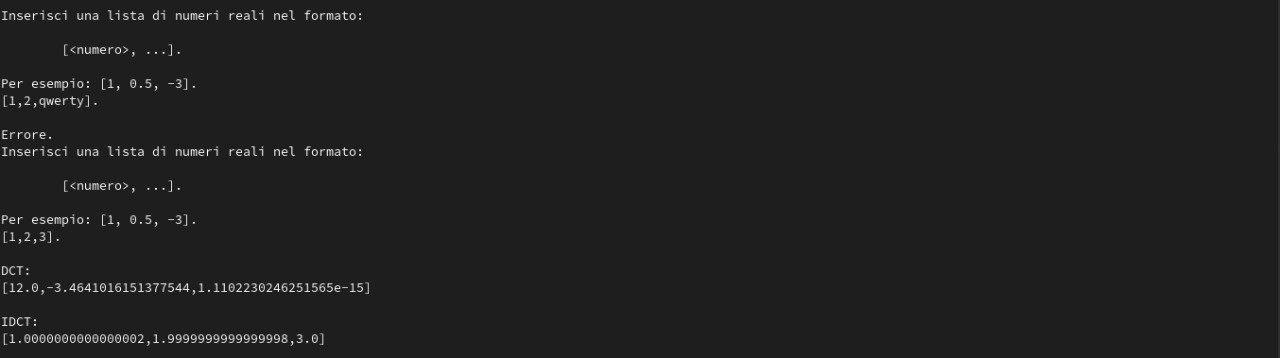
\includegraphics[width=\textwidth]{test_pl_5.jpg}
        \caption{Tipo in input errato durante l'inserimento per DCT}
      \end{figure}
    \end{center}

    \begin{center}
      \begin{figure}
        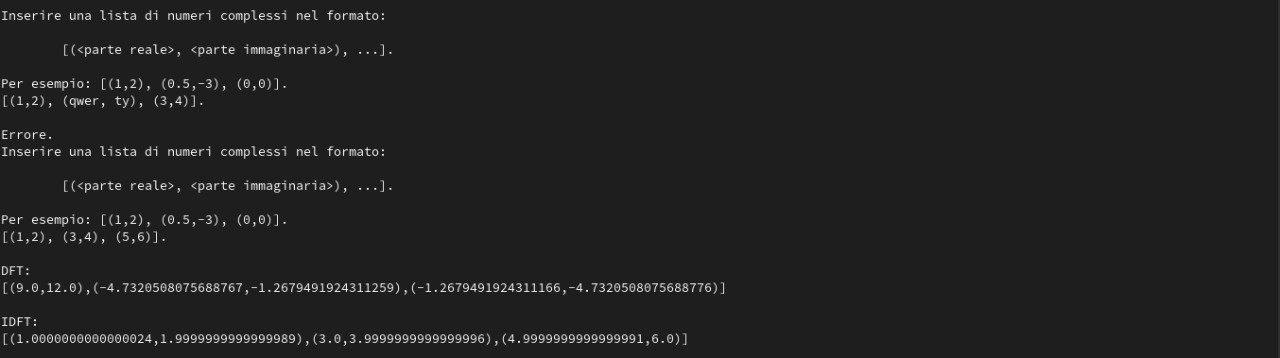
\includegraphics[width=\textwidth]{test_pl_6.jpg}
        \caption{Tipo in input errato durante l'inserimento per DFT}
      \end{figure}
    \end{center}

     \begin{center}
       \begin{figure}
         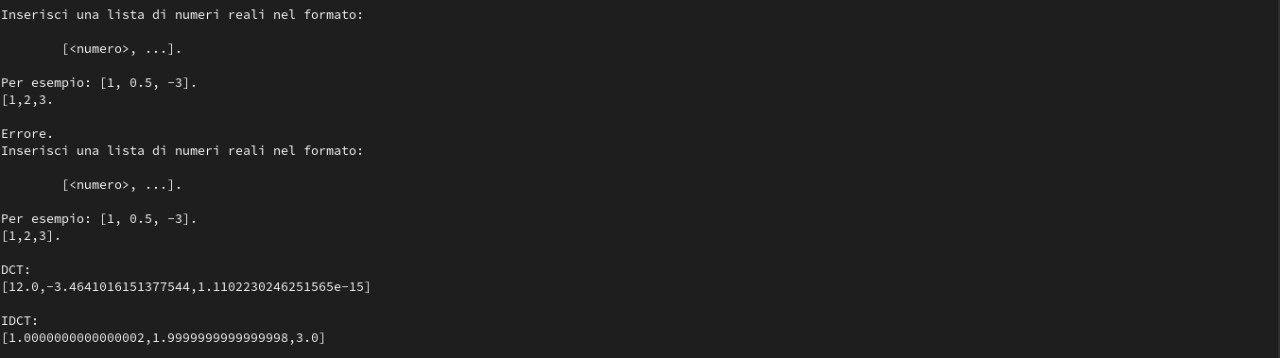
\includegraphics[width=\textwidth]{test_pl_7.jpg}
         \caption{Formattazione errata durante l'inserimento per DCT}
       \end{figure}
     \end{center}

     \begin{center}
       \begin{figure}
         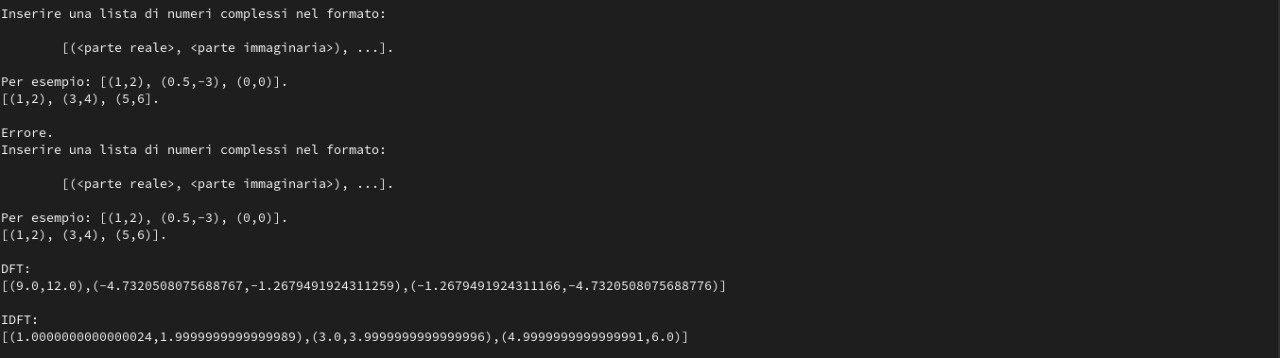
\includegraphics[width=\textwidth]{test_pl_8.jpg}
         \caption{Formattazione errata durante l'inserimento per DFT}
       \end{figure}
     \end{center}

     \begin{center}
       \begin{figure}
         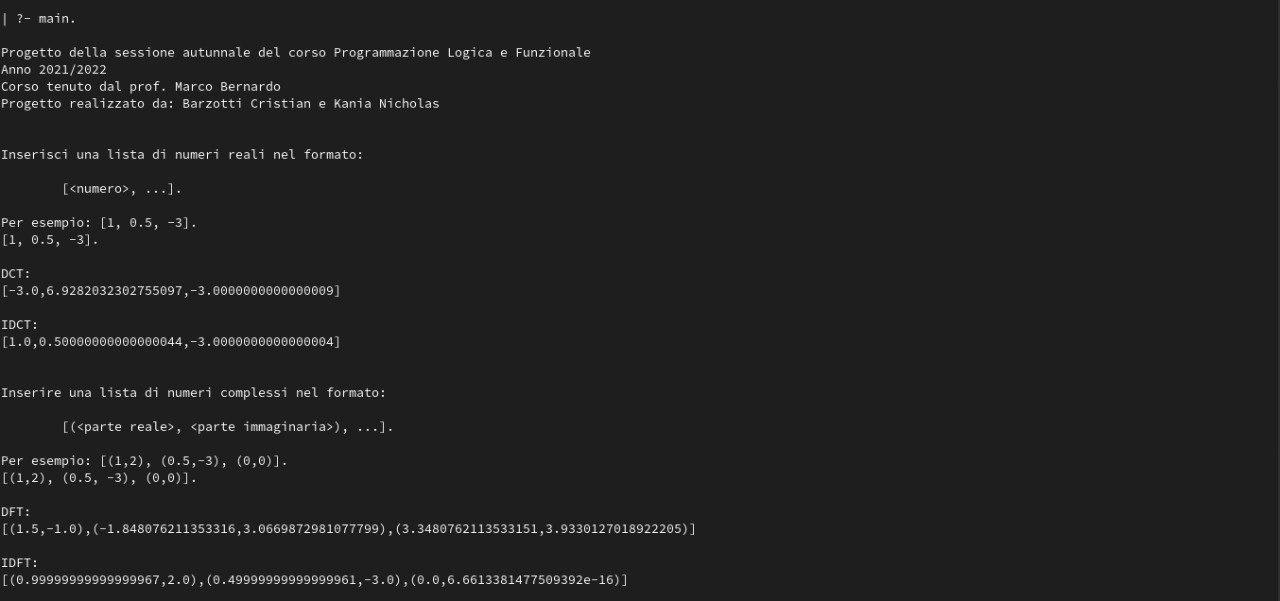
\includegraphics[width=\textwidth]{test_pl_9.jpg}
         \caption{Funzionamento dell'intero programma con input corretti}
       \end{figure}
     \end{center}

     \begin{center}
       \begin{figure}
         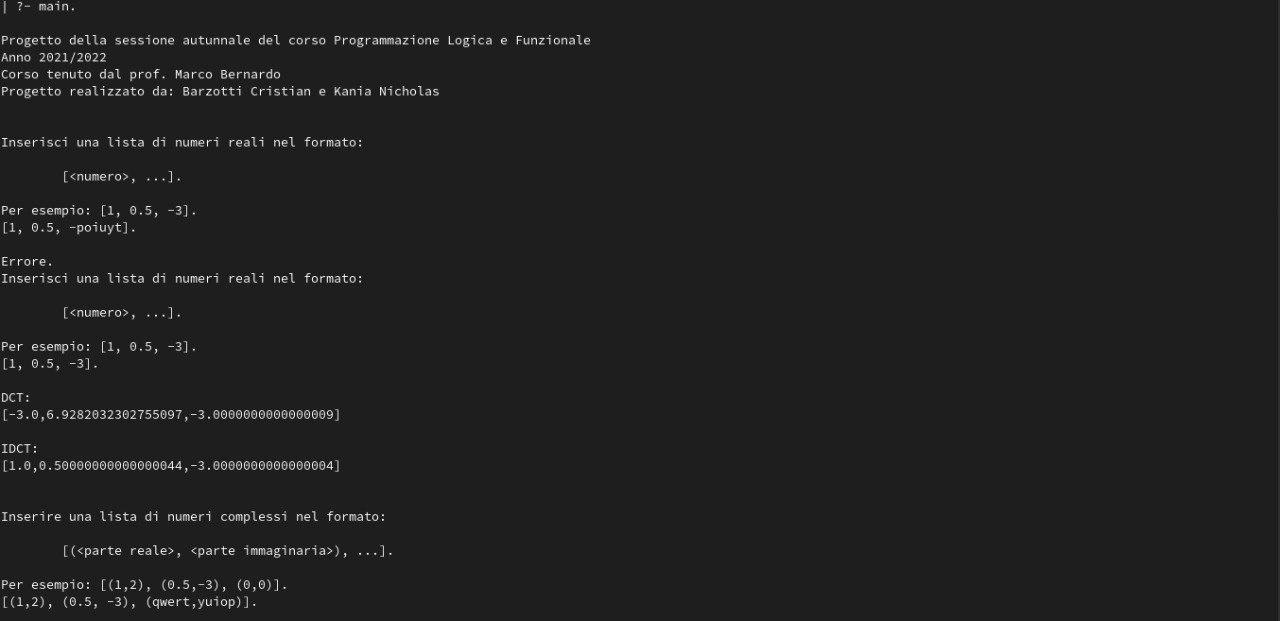
\includegraphics[width=\textwidth]{test_pl_10a.jpg}
         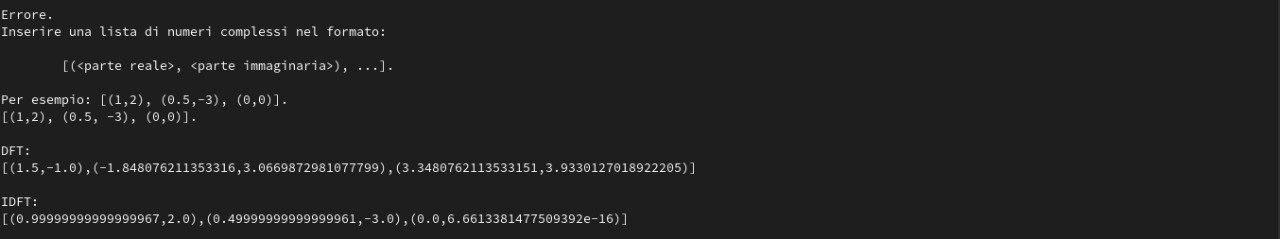
\includegraphics[width=\textwidth]{test_pl_10b.jpg}
         \caption{Funzionamento dell'intero programma con alcuni input errati}
       \end{figure}
     \end{center}
\end{document}